\documentclass{article}

\title{Report}
%\date{}
\author{Siddharth Nayak EE16B073 }
\usepackage{graphicx}
\usepackage{hyperref}
\usepackage{amsmath}
\usepackage{amsfonts}
\usepackage{amssymb}
\usepackage{float}
\usepackage{geometry}
\geometry{legalpaper, portrait, margin=1in}
\newcommand\tab[1][1cm]{\hspace*{#1}}
\newcommand \Mycomb[2][^n]{\prescript{#1\mkern-0.5mu}{}C_{#2}}

 \hypersetup{
    colorlinks=true,
    linkcolor=blue,
    filecolor=magenta,      
    urlcolor=blue,
}
 
\urlstyle{same}
 
\begin{document}

\maketitle
\newcommand{\norm}[1]{\left\lVert#1\right\rVert}
\pagenumbering{arabic}

\section{Part 1: Visualisation of images}:

\begin{figure}[H]
\subfigure{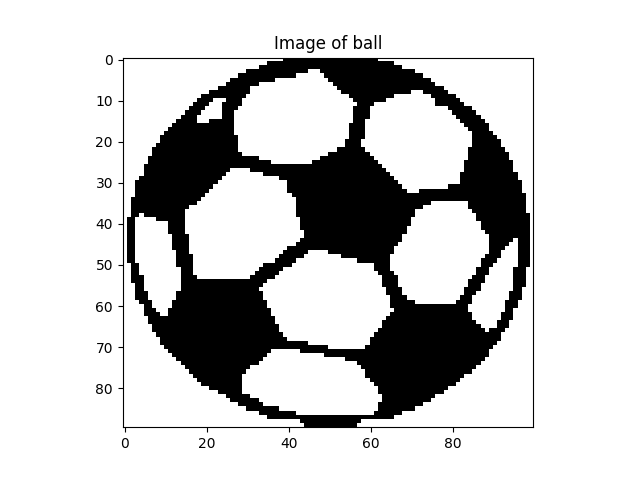
\includegraphics[width=0.55\textwidth]{Figure_1.png}}
%\hspace{0.001\textwidth}
\subfigure{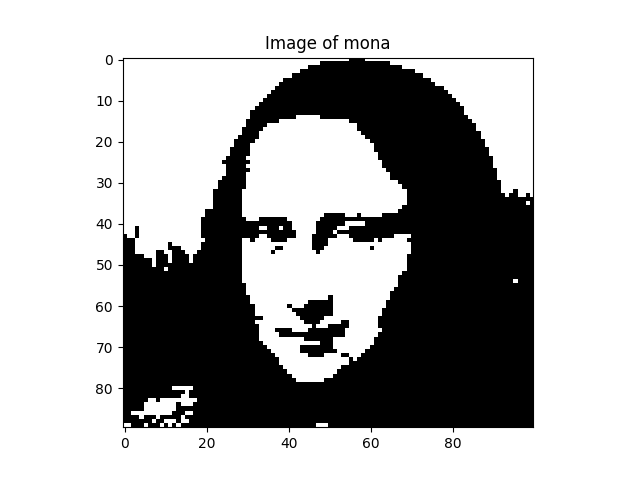
\includegraphics[width=0.55\textwidth]{Figure_2.png}}
\end{figure}

\begin{figure}[H]
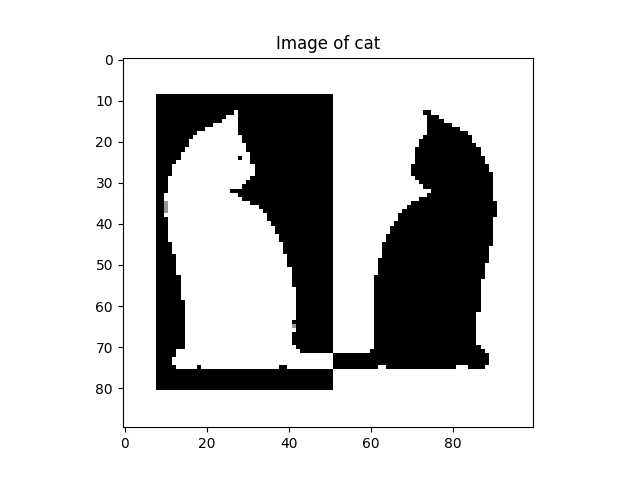
\includegraphics[width=0.55\textwidth]{Figure_3.png}
\centering
\end{figure}

\section{Part 2: }
Now the image of the football is saved in the network. The weights are not perturbed (set to zero). Then a patch of the original image is given as the input. The original image is retrieved back by the network as follows:
\begin{figure}[H]
\subfigure{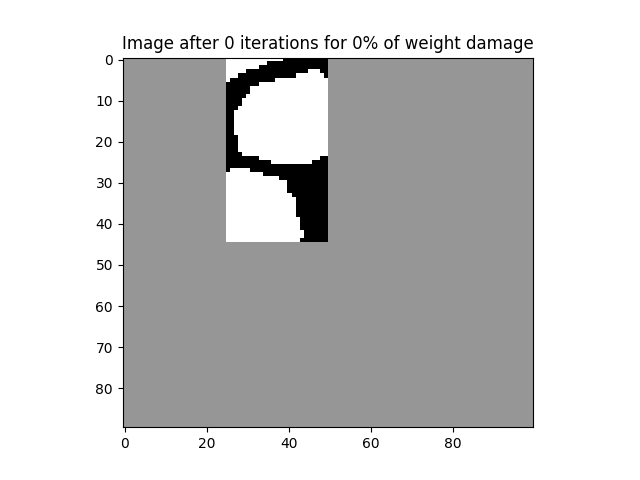
\includegraphics[width=0.55\textwidth]{Figure_10.png}}
\hspace{0.001\textwidth}
\subfigure{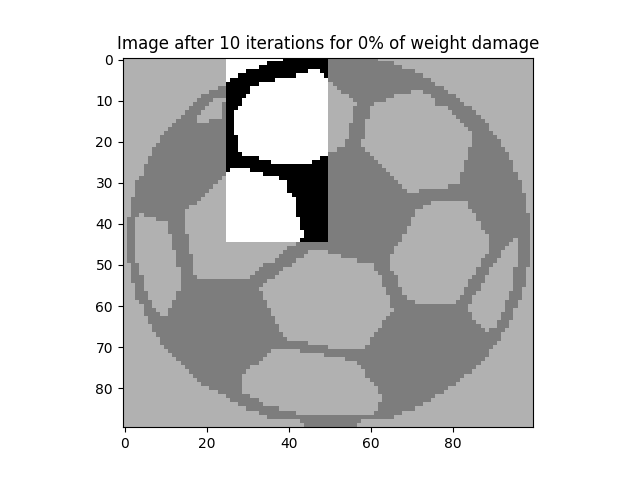
\includegraphics[width=0.55\textwidth]{Figure_11.png}}
\end{figure}

\begin{figure}[H]
\subfigure{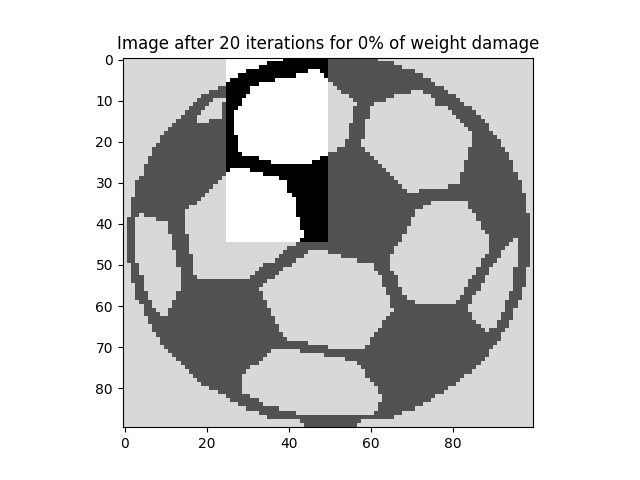
\includegraphics[width=0.55\textwidth]{Figure_12.png}}
\hspace{0.001\textwidth}
\subfigure{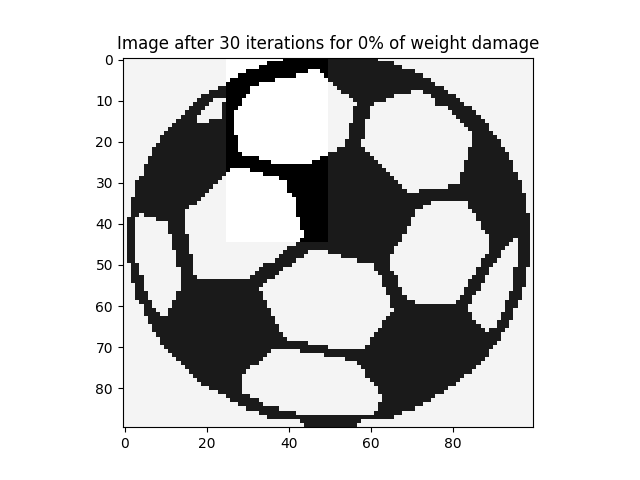
\includegraphics[width=0.55\textwidth]{Figure_13.png}}
\end{figure}

\begin{figure}[H]
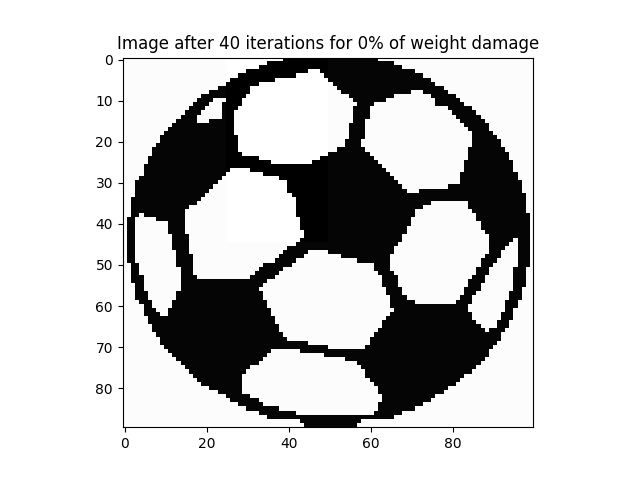
\includegraphics[width=0.55\textwidth]{Figure_14.png}
\centering
\end{figure}


The Root mean Square of the change in the network is plotted with respect to number of iterations. Initially there is a linear decrease in the loss and then after 20 iterations there is an exponential decrease in the loss.
\begin{figure}[H]
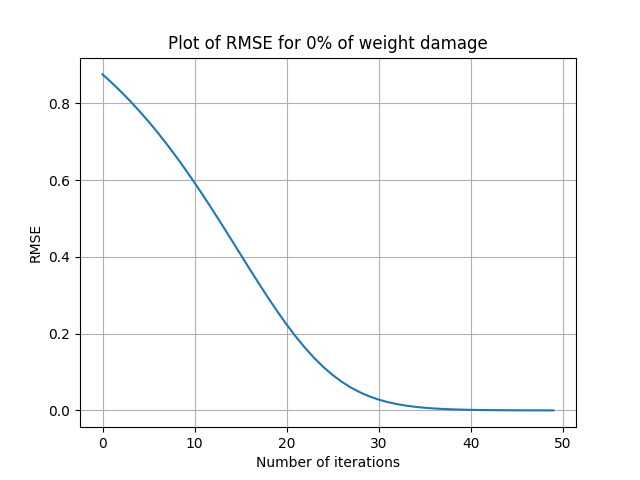
\includegraphics[width=0.55\textwidth]{Figure_15.png}
\centering
\end{figure}

\section{Part 3:}
Now all three images are loaded into the network,(Cat, Mona Lisa and Ball). Then the weights are perturbed (set to zero) with some probability 'p'. Then a patch of the image of the ball is given as the trigger. This will make the initial retrievals a little hazy(has hallucinations of Mona Lisa and the cat) because of the presence of the other images in the network as well as the weights being disturbed. But after some number of iterations there is almost no difference between the original and the retrieved image. The amount of hallucinations as well as the number of iterations required to get almost similar image depends on the percentage of weights disturbed.

\subsection{25\% weight damage}
\begin{figure}[H]
\subfigure{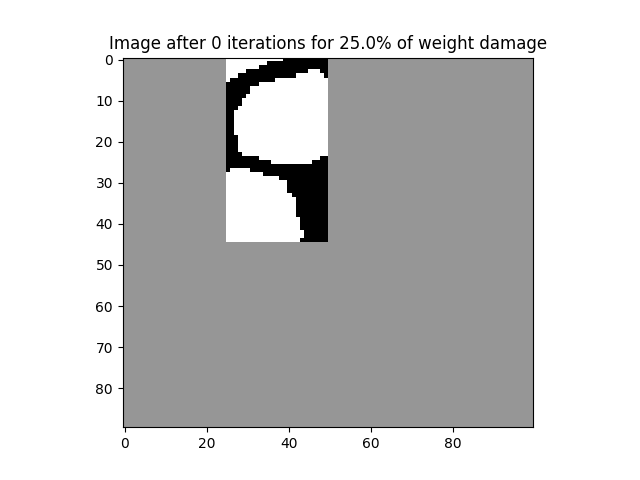
\includegraphics[width=0.55\textwidth]{Figure_20.png}}
\hspace{0.001\textwidth}
\subfigure{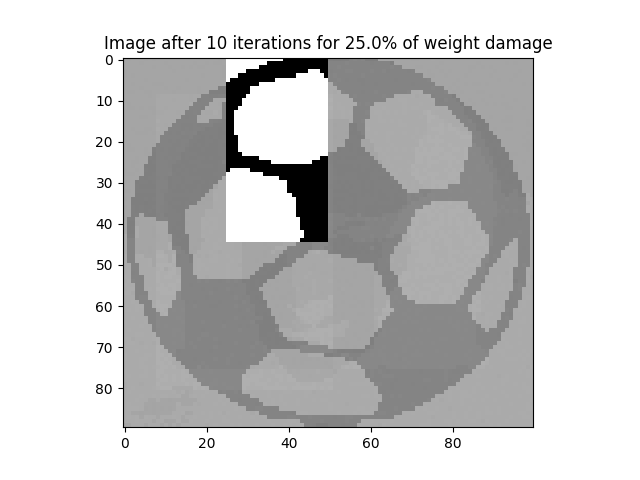
\includegraphics[width=0.55\textwidth]{Figure_21.png}}
\end{figure}

\begin{figure}[H]
\subfigure{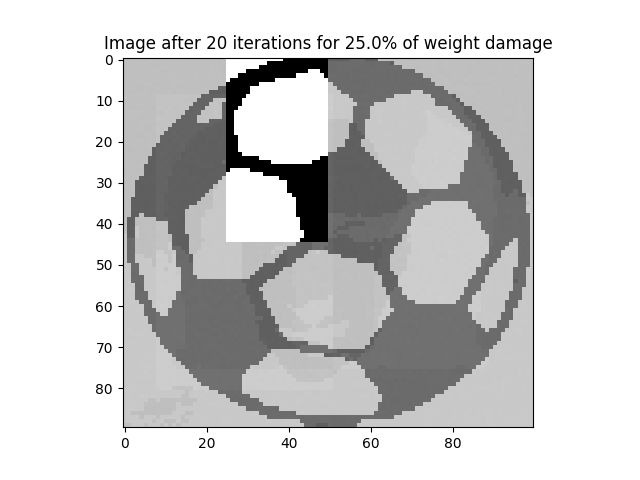
\includegraphics[width=0.55\textwidth]{Figure_22.png}}
\hspace{0.001\textwidth}
\subfigure{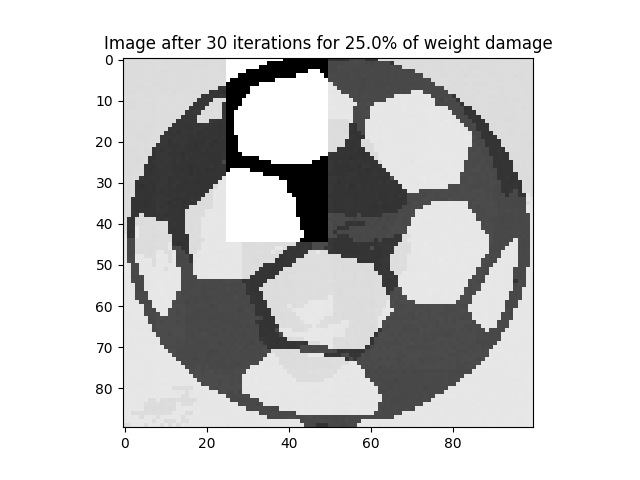
\includegraphics[width=0.55\textwidth]{Figure_23.png}}
\end{figure}

\begin{figure}[H]
\subfigure{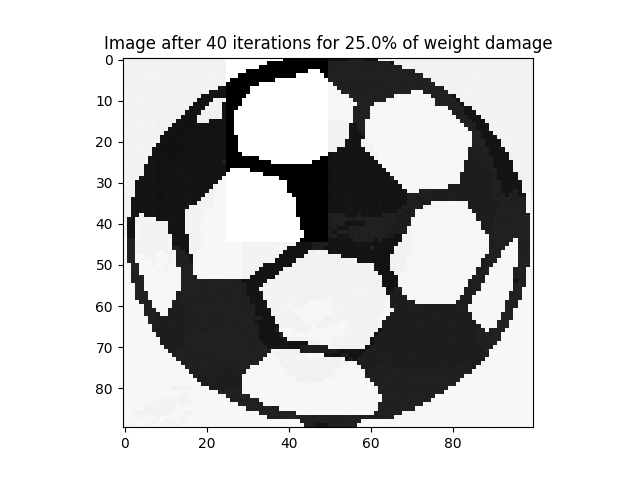
\includegraphics[width=0.55\textwidth]{Figure_24.png}}
\hspace{0.001\textwidth}
\subfigure{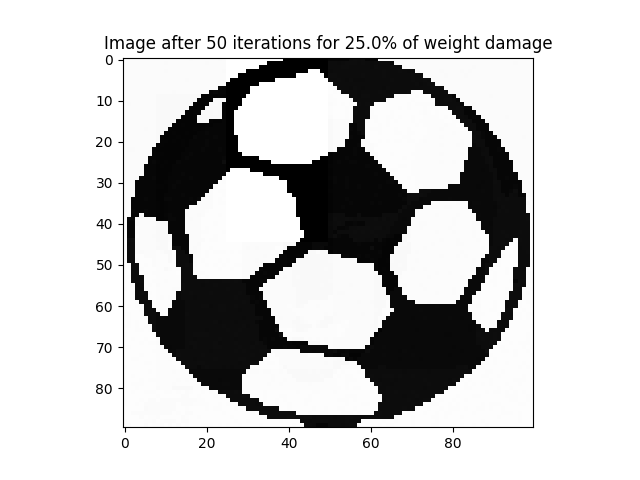
\includegraphics[width=0.55\textwidth]{Figure_25.png}}
\end{figure}

\begin{figure}[H]
\subfigure{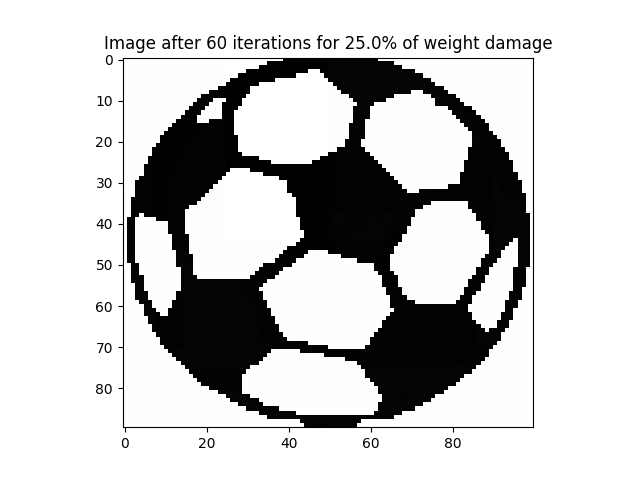
\includegraphics[width=0.55\textwidth]{Figure_26.png}}
\hspace{0.001\textwidth}
\subfigure{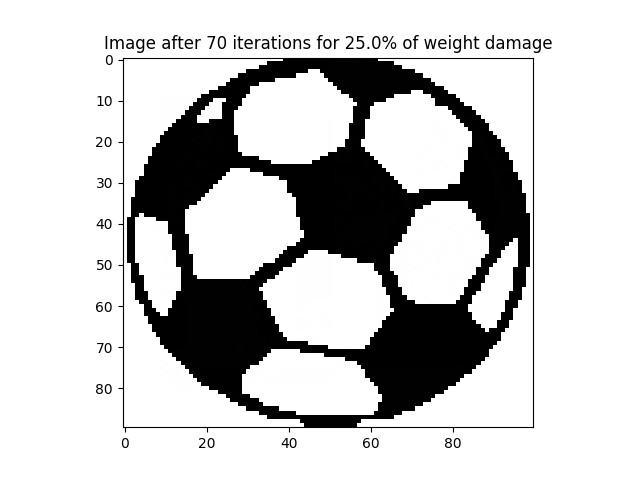
\includegraphics[width=0.55\textwidth]{Figure_27.png}}
\end{figure}

\begin{figure}[H]
\subfigure{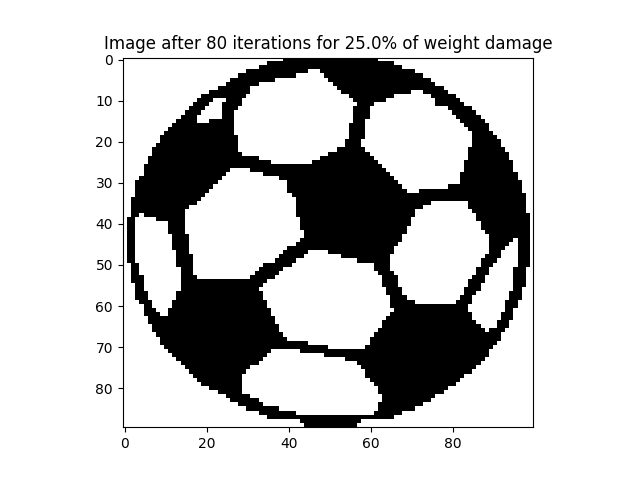
\includegraphics[width=0.55\textwidth]{Figure_28.png}}
\hspace{0.001\textwidth}
\subfigure{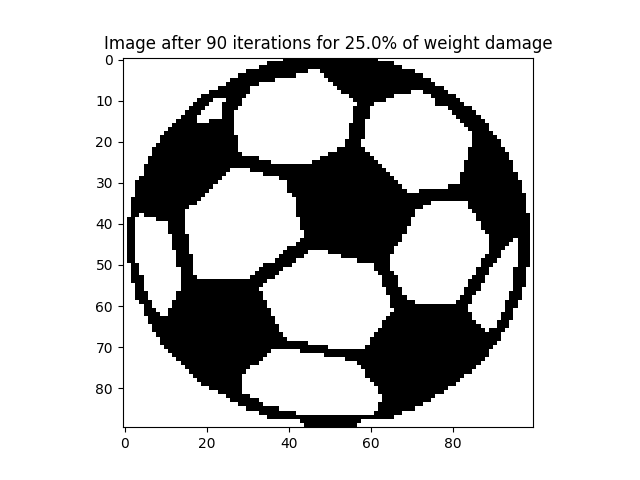
\includegraphics[width=0.55\textwidth]{Figure_29.png}}
\end{figure}

The Root mean Square of the change in the network is plotted with respect to number of iterations. Initially there is a linear decrease in the loss and then after 30 iterations there is an exponential decrease in the loss.
\begin{figure}[H]
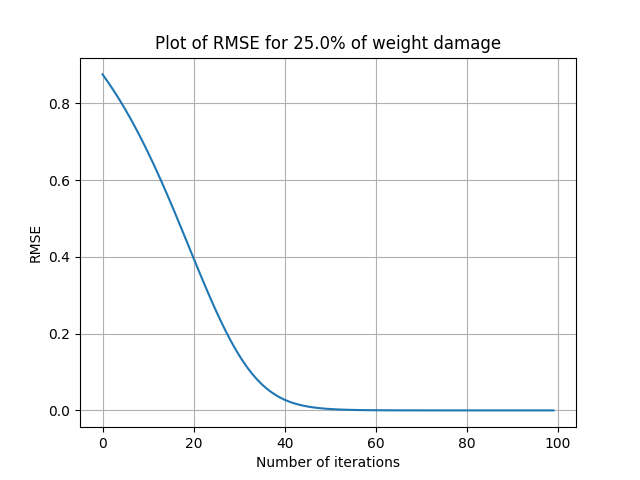
\includegraphics[width=0.55\textwidth]{Figure_211.png}
\centering
\end{figure}

\subsection{50\% weight damage}
\begin{figure}[H]
\subfigure{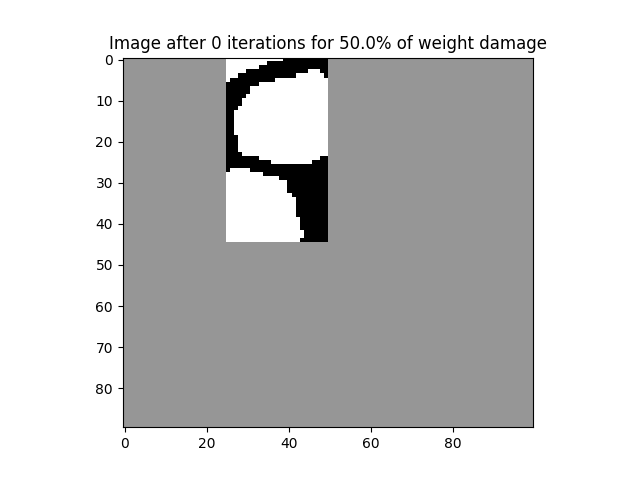
\includegraphics[width=0.55\textwidth]{Figure_30.png}}
\hspace{0.001\textwidth}
\subfigure{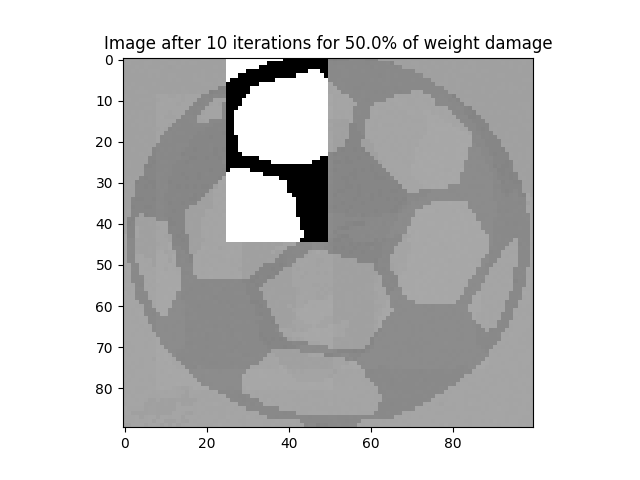
\includegraphics[width=0.55\textwidth]{Figure_31.png}}
\end{figure}

\begin{figure}[H]
\subfigure{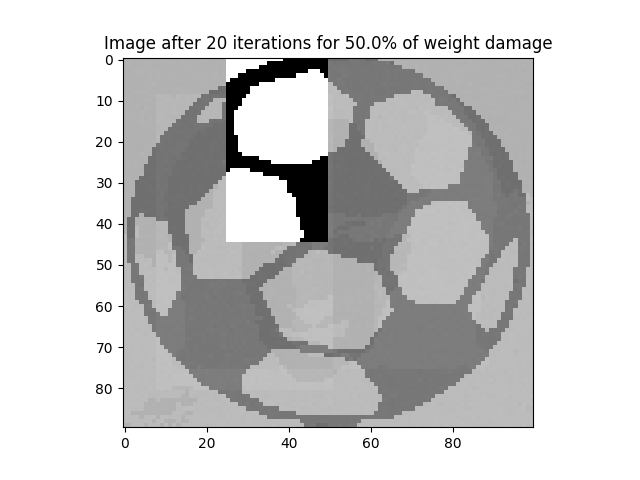
\includegraphics[width=0.55\textwidth]{Figure_32.png}}
\hspace{0.001\textwidth}
\subfigure{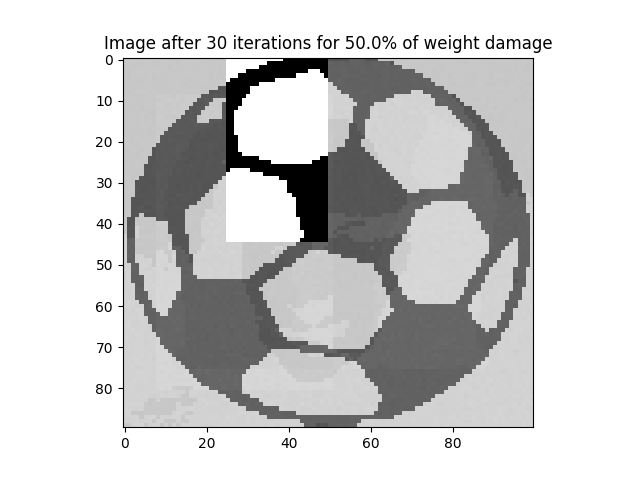
\includegraphics[width=0.55\textwidth]{Figure_33.png}}
\end{figure}

\begin{figure}[H]
\subfigure{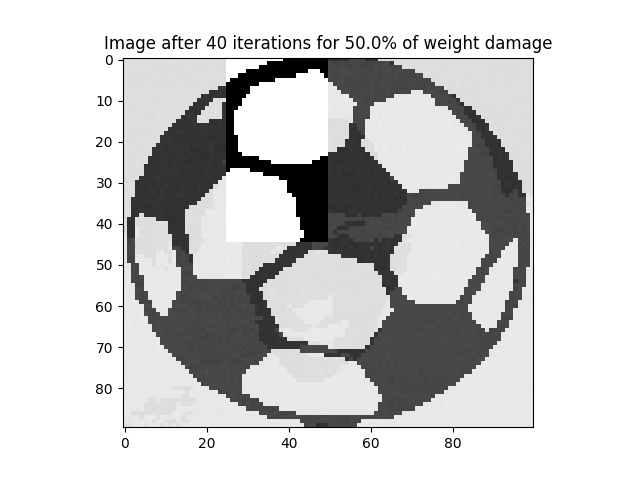
\includegraphics[width=0.55\textwidth]{Figure_34.png}}
\hspace{0.001\textwidth}
\subfigure{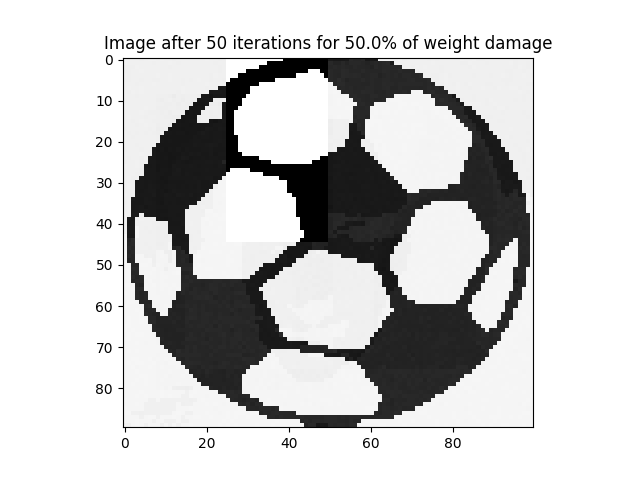
\includegraphics[width=0.55\textwidth]{Figure_35.png}}
\end{figure}

\begin{figure}[H]
\subfigure{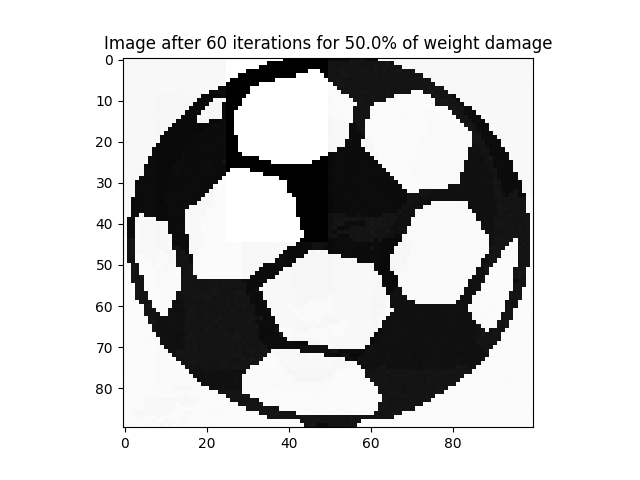
\includegraphics[width=0.55\textwidth]{Figure_36.png}}
\hspace{0.001\textwidth}
\subfigure{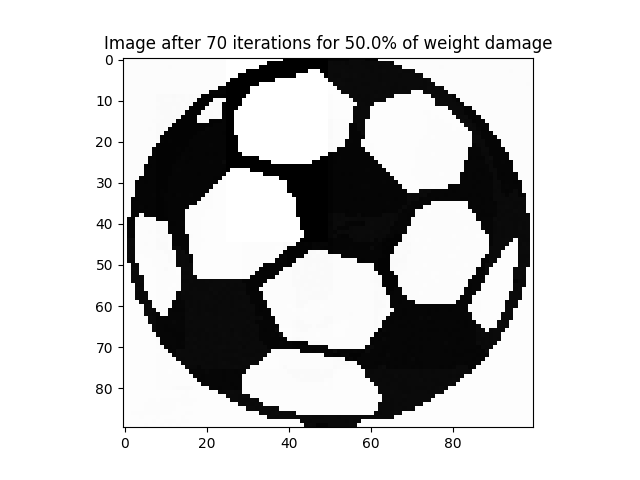
\includegraphics[width=0.55\textwidth]{Figure_37.png}}
\end{figure}

\begin{figure}[H]
\subfigure{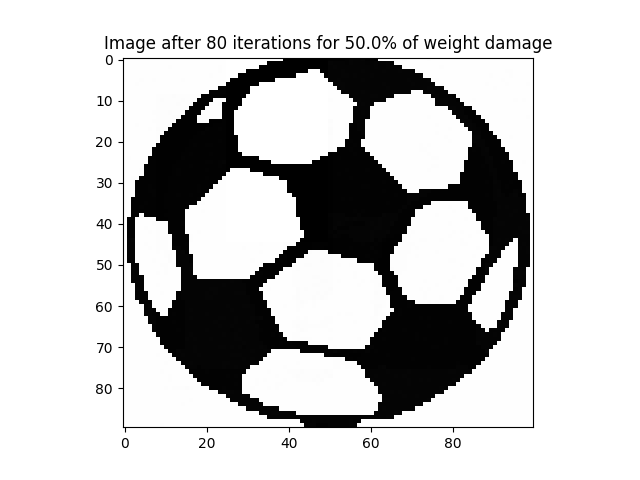
\includegraphics[width=0.55\textwidth]{Figure_38.png}}
\hspace{0.001\textwidth}
\subfigure{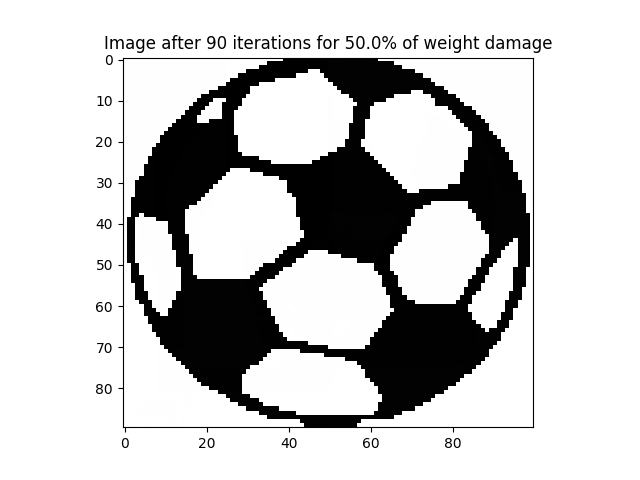
\includegraphics[width=0.55\textwidth]{Figure_39.png}}
\end{figure}

The Root mean Square of the change in the network is plotted with respect to number of iterations. Initially there is a linear decrease in the loss and then after 35 iterations there is an exponential decrease in the loss.
\begin{figure}[H]
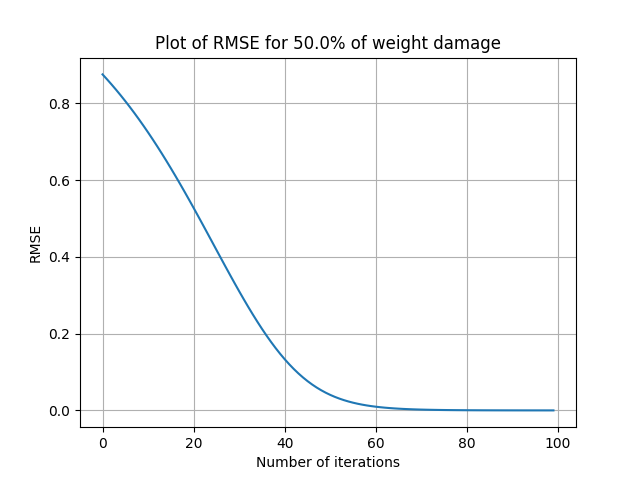
\includegraphics[width=0.55\textwidth]{Figure_311.png}
\centering
\end{figure}

\subsection{80\% weight damage}
\begin{figure}[H]
\subfigure{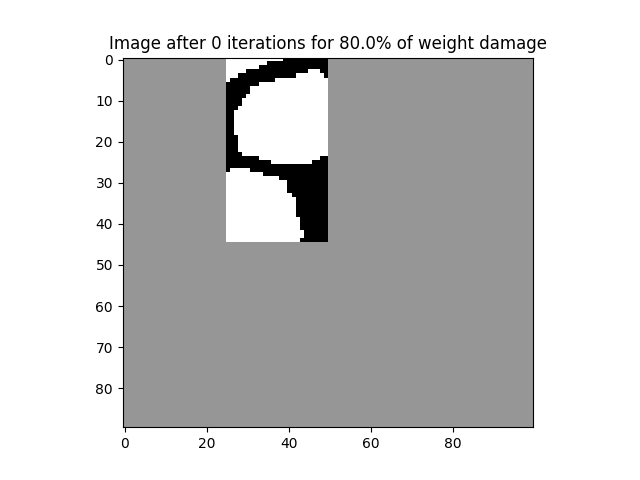
\includegraphics[width=0.55\textwidth]{Figure_40.png}}
\hspace{0.001\textwidth}
\subfigure{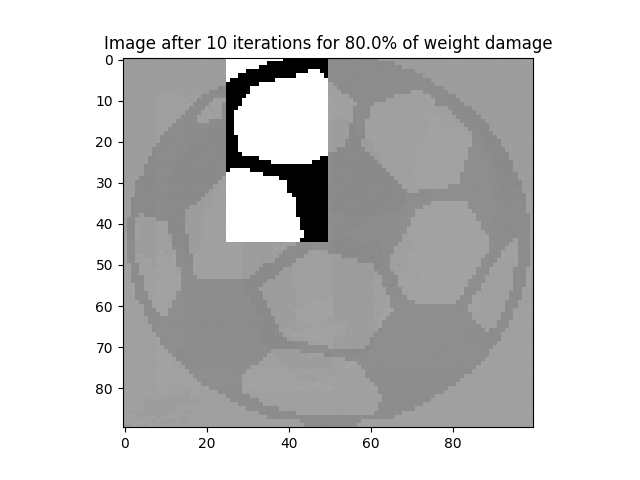
\includegraphics[width=0.55\textwidth]{Figure_41.png}}
\end{figure}

\begin{figure}[H]
\subfigure{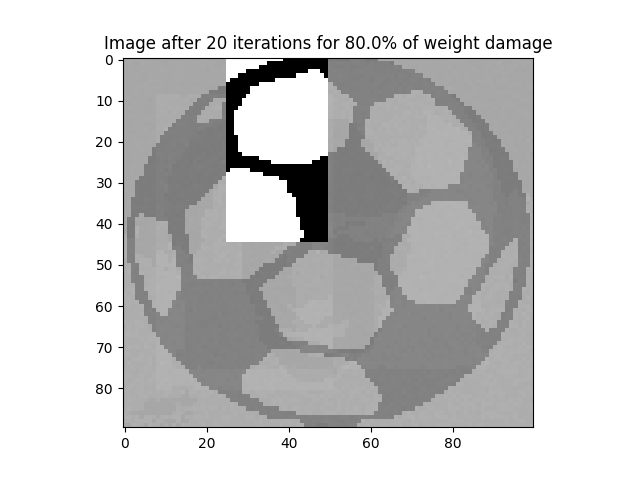
\includegraphics[width=0.55\textwidth]{Figure_42.png}}
\hspace{0.001\textwidth}
\subfigure{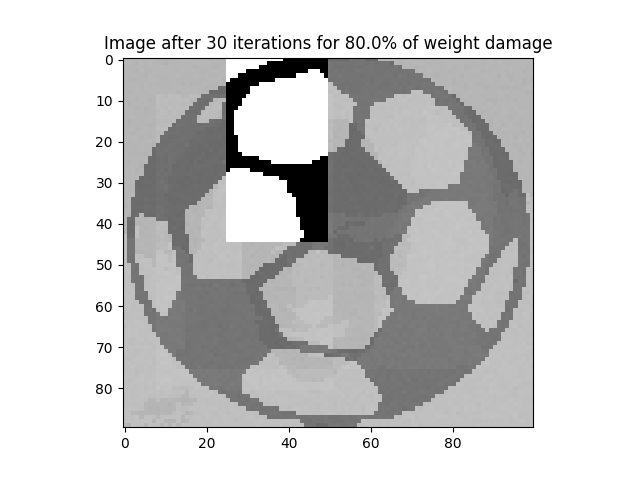
\includegraphics[width=0.55\textwidth]{Figure_43.png}}
\end{figure}

\begin{figure}[H]
\subfigure{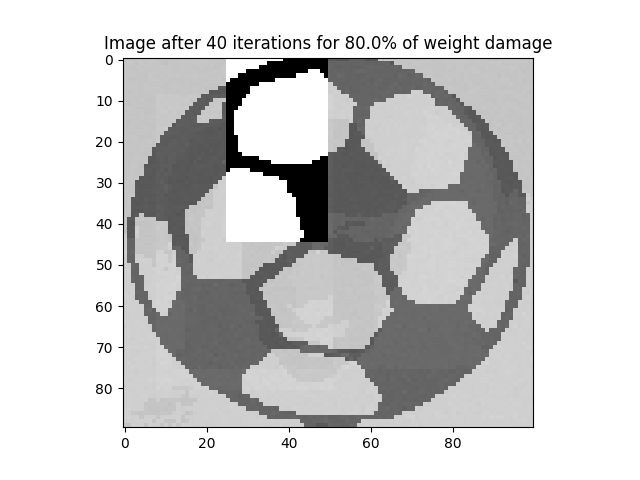
\includegraphics[width=0.55\textwidth]{Figure_44.png}}
\hspace{0.001\textwidth}
\subfigure{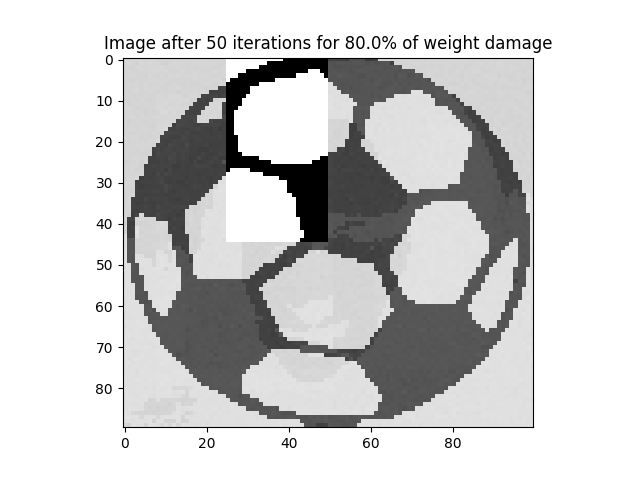
\includegraphics[width=0.55\textwidth]{Figure_45.png}}
\end{figure}

\begin{figure}[H]
\subfigure{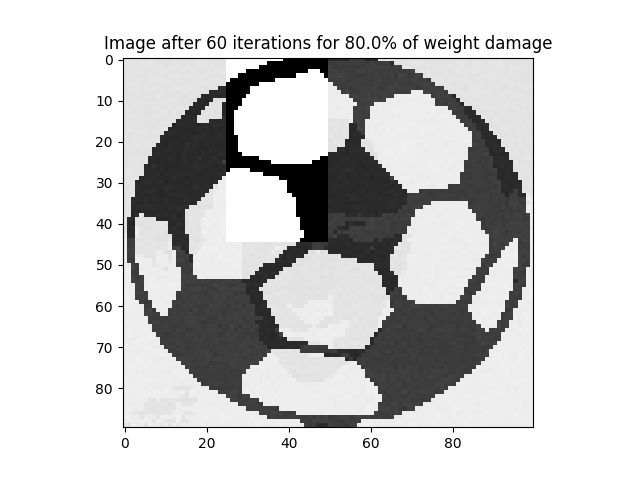
\includegraphics[width=0.55\textwidth]{Figure_46.png}}
\hspace{0.001\textwidth}
\subfigure{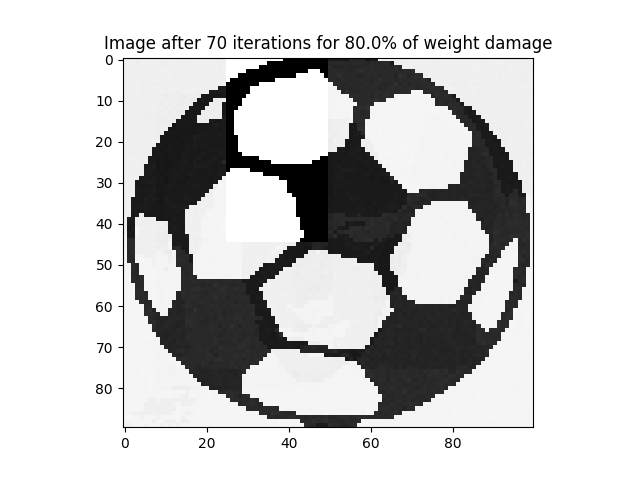
\includegraphics[width=0.55\textwidth]{Figure_47.png}}
\end{figure}

\begin{figure}[H]
\subfigure{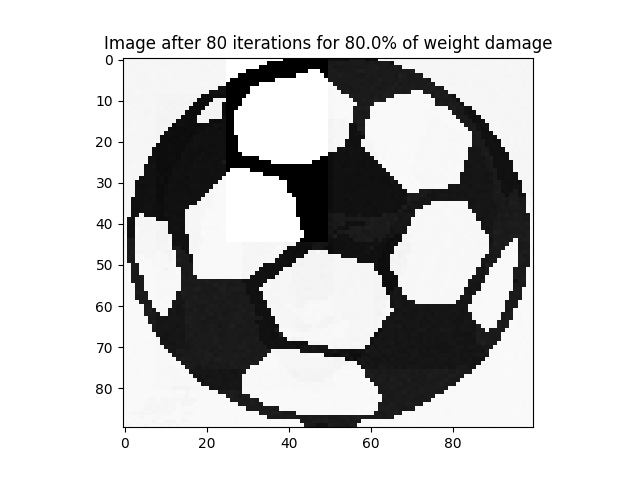
\includegraphics[width=0.55\textwidth]{Figure_48.png}}
\hspace{0.001\textwidth}
\subfigure{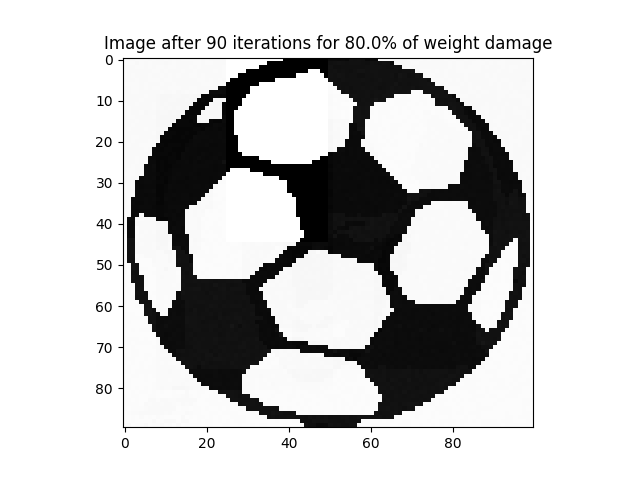
\includegraphics[width=0.55\textwidth]{Figure_49.png}}
\end{figure}

The Root mean Square of the change in the network is plotted with respect to number of iterations. Initially there is a linear decrease in the loss and then after 45 iterations there is an exponential decrease in the loss.
\begin{figure}[H]
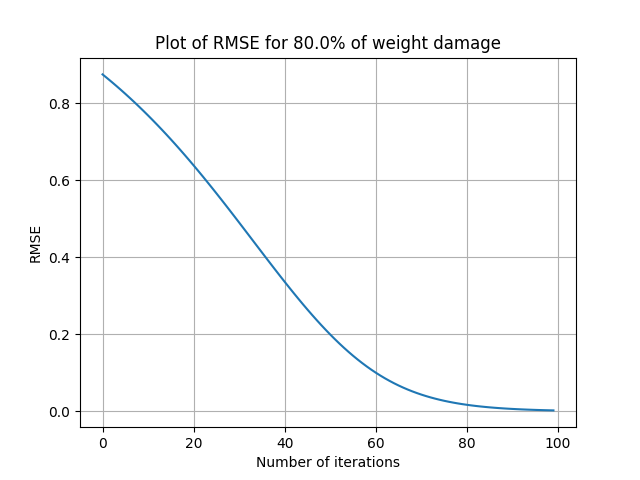
\includegraphics[width=0.55\textwidth]{Figure_411.png}
\centering
\end{figure}

%%%%%%%%%%%%%%%%%%%%%%%%%%%%%%%%%%%%%%%%%%%%%%%%%%%%%%%%%%%%%%%%%%%%%%%%%%%%%%%%%%%%%%%%%%%%%%%%%%%%%%%%%%%%%%%%%%%%%%

\section{Mona Lisa as the input}
\begin{figure}[H]
\subfigure{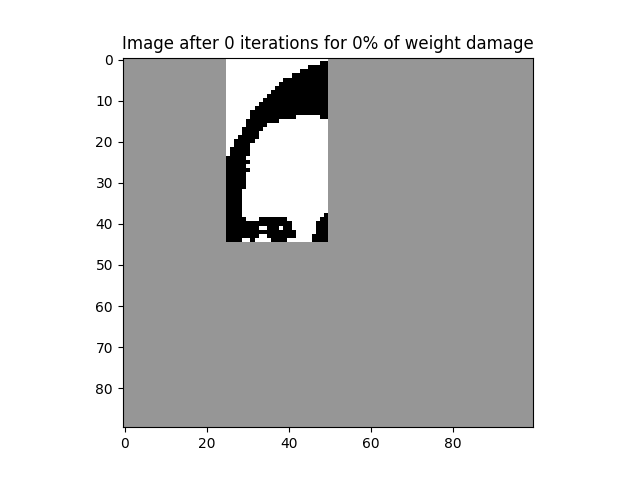
\includegraphics[width=0.55\textwidth]{Mona_init.png}}
\hspace{0.001\textwidth}
\subfigure{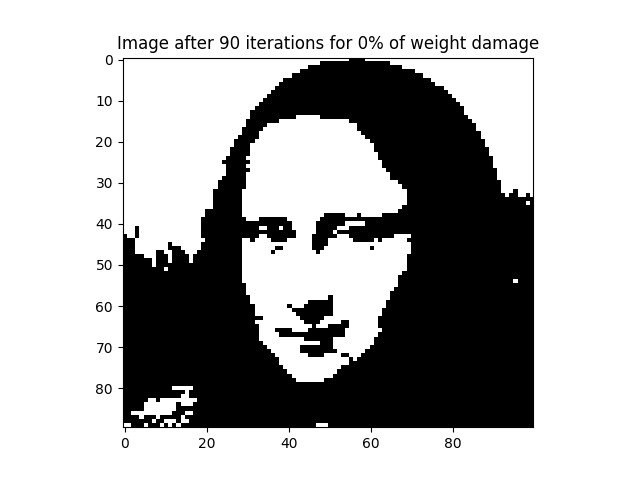
\includegraphics[width=0.55\textwidth]{Mona_final.png}}
\end{figure}


The Root mean Square of the change in the network is plotted with respect to number of iterations. Initially there is a linear decrease in the loss and then after 20 iterations there is an exponential decrease in the loss.
\begin{figure}[H]
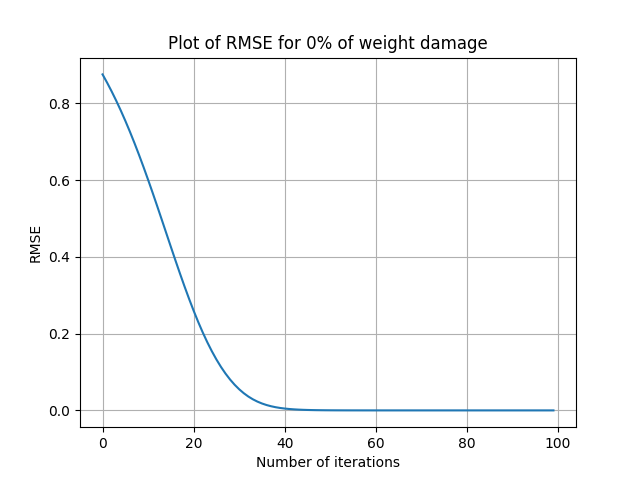
\includegraphics[width=0.55\textwidth]{Mona_loss.png}
\centering
\end{figure}

\begin{figure}[H]
\subfigure{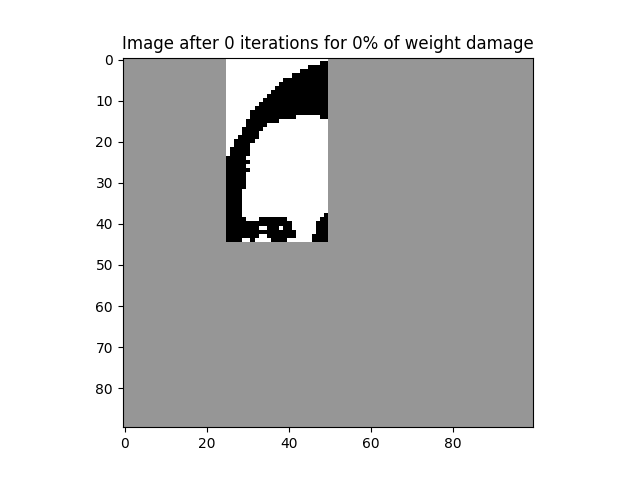
\includegraphics[width=0.55\textwidth]{Mona1.png}}
\hspace{0.001\textwidth}
\subfigure{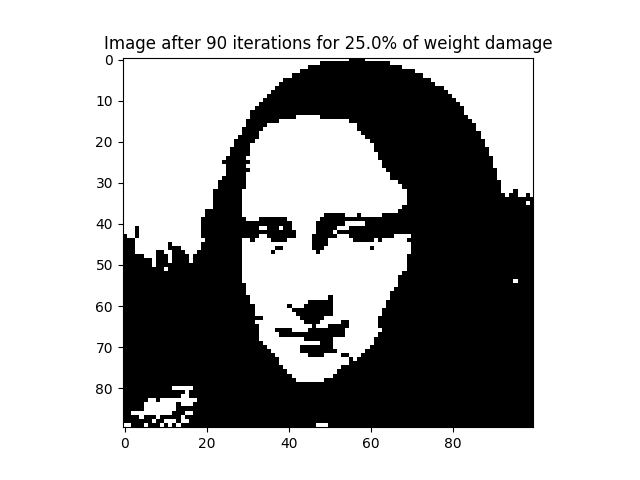
\includegraphics[width=0.55\textwidth]{Mona_21.png}}
\end{figure}


The Root mean Square of the change in the network is plotted with respect to number of iterations. Initially there is a linear decrease in the loss and then after 30 iterations there is an exponential decrease in the loss.
\begin{figure}[H]
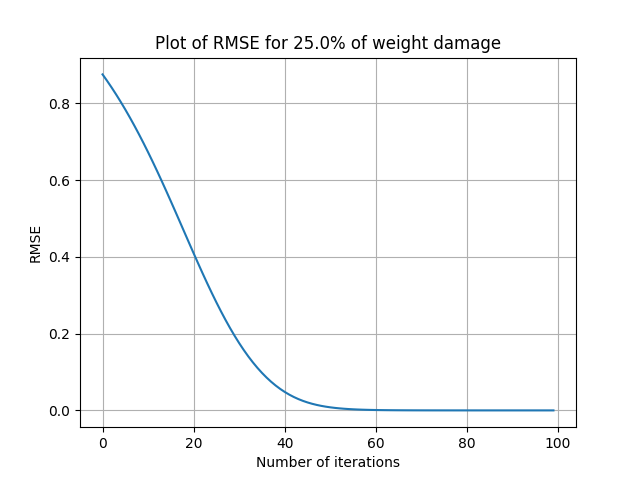
\includegraphics[width=0.55\textwidth]{Mona_22.png}
\centering
\end{figure}

\begin{figure}[H]
\subfigure{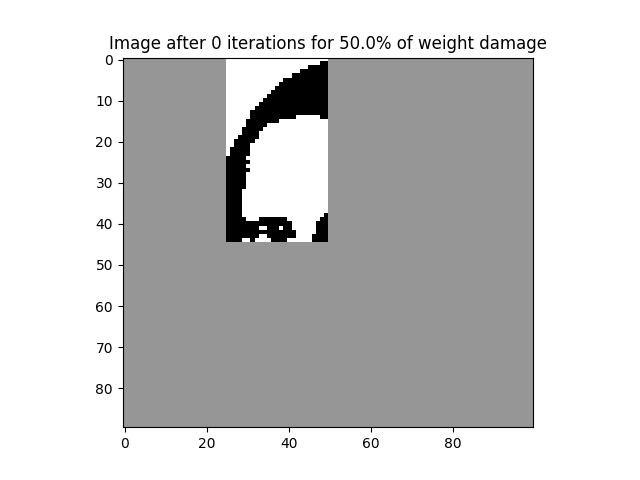
\includegraphics[width=0.55\textwidth]{Mona_30.png}}
\hspace{0.001\textwidth}
\subfigure{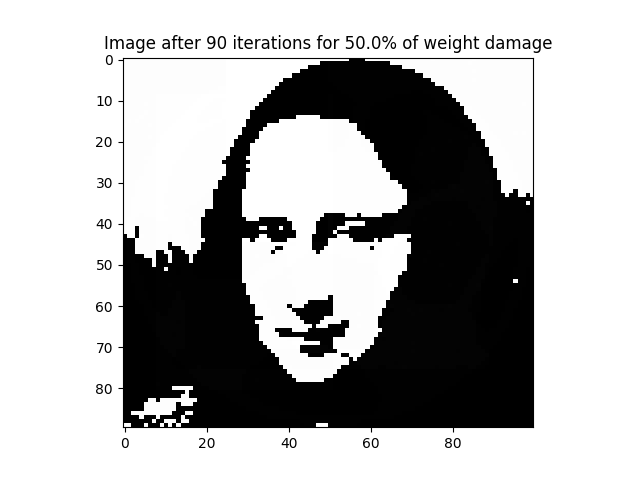
\includegraphics[width=0.55\textwidth]{Mona_31.png}}
\end{figure}


The Root mean Square of the change in the network is plotted with respect to number of iterations. Initially there is a linear decrease in the loss and then after 40 iterations there is an exponential decrease in the loss.
\begin{figure}[H]
\includegraphics[width=0.55\textwidth]{Mona_33.png}
\centering
\end{figure}

\begin{figure}[H]
\subfigure{\includegraphics[width=0.55\textwidth]{Mona_40.png}}
\hspace{0.001\textwidth}
\subfigure{\includegraphics[width=0.55\textwidth]{Mona_41.png}}
\end{figure}


The Root mean Square of the change in the network is plotted with respect to number of iterations. Initially there is a linear decrease in the loss and then after 50 iterations there is an exponential decrease in the loss.
\begin{figure}[H]
\includegraphics[width=0.55\textwidth]{Mona_43.png}
\centering
\end{figure}

%%%%%%%%%%%%%%%%%%%%%%%%%%%%%%%%%%%%%%%%%%%%%%%%%%%%%%%%%%%%%%%%%%%%%%%%%%%%%%%%%%%%%%%%%%%%%%%%%%%%%%%%%%%%%%%%%%%%%%

\section{Cat as the input}
\begin{figure}[H]
\subfigure{\includegraphics[width=0.55\textwidth]{Cat_init.png}}
\hspace{0.001\textwidth}
\subfigure{\includegraphics[width=0.55\textwidth]{cat_final.png}}
\end{figure}


The Root mean Square of the change in the network is plotted with respect to number of iterations. Initially there is a linear decrease in the loss and then after 30 iterations there is an exponential decrease in the loss.
\begin{figure}[H]
\includegraphics[width=0.55\textwidth]{cat_loss.png}
\centering
\end{figure}

\begin{figure}[H]
\subfigure{\includegraphics[width=0.55\textwidth]{cat_10.png}}
\hspace{0.001\textwidth}
\subfigure{\includegraphics[width=0.55\textwidth]{cat_11.png}}
\end{figure}


The Root mean Square of the change in the network is plotted with respect to number of iterations. Initially there is a linear decrease in the loss and then after 30 iterations there is an exponential decrease in the loss.
\begin{figure}[H]
\includegraphics[width=0.55\textwidth]{cat_12.png}
\centering
\end{figure}

\begin{figure}[H]
\subfigure{\includegraphics[width=0.55\textwidth]{cat_20.png}}
\hspace{0.001\textwidth}
\subfigure{\includegraphics[width=0.55\textwidth]{cat_21.png}}
\end{figure}


The Root mean Square of the change in the network is plotted with respect to number of iterations. Initially there is a linear decrease in the loss and then after 30 iterations there is an exponential decrease in the loss.
\begin{figure}[H]
\includegraphics[width=0.55\textwidth]{cat_22.png}
\centering
\end{figure}1

\begin{figure}[H]
\subfigure{\includegraphics[width=0.55\textwidth]{cat_40.png}}
\hspace{0.001\textwidth}
\subfigure{\includegraphics[width=0.55\textwidth]{cat_41.png}}
\end{figure}


The Root mean Square of the change in the network is plotted with respect to number of iterations. Initially there is a linear decrease in the loss and then after 30 iterations there is an exponential decrease in the loss.
\begin{figure}[H]
\includegraphics[width=0.55\textwidth]{cat_42.png}
\centering
\end{figure}

\section{Conclusions}
The images stored in the Hopfield Network are retrieved back by giving in suitable inputs (triggers). Thus showing the effectiveness of the Network to remember the stored images even after damaging the weights.
%%%%%%%%%%%%%%%%%%%%%%%%%%%%%%%%%%%%%%%%%%%%%%%%%%%%%%%%%%%%%%%%%%%%%%%%%%%%%%%%%%%%%%%%%%%%%%%%%%%%%%%%%%%%%%%%%%%%%%
\end{document}
